\section{Validation}
\label{appendix.validation}

\subsection{OCL Constraints}
All the constraints described bellow apply to the \emph{Bicycle} context! 

\begin{table}[htp]
\begin{center}
	\rowcolors{1}{white}{lightgray}
	\lstset{captionpos=b,language=OCL,numbers=none,basicstyle=\small}
	\lstset{linewidth=.7\textwidth}
	\begin{tabular*}{\textwidth}{p{.015\textwidth} p{.3\textwidth} l}
	\hline \hline
\textbf{No} & \textbf{Description} & \textbf{Constraint} \\ \hline \hline
1	&	It has one or two wheels &
\begin{lstlisting}
self.parts->select(oclIsTypeOf(Wheel))->size() > 0 and 
self.parts->select(oclIsTypeOf(Wheel))->size() < 3
\end{lstlisting}  \\ 

2	&	It can have an outer gear if it has two wheels and does not have an inner gear &
\begin{lstlisting}
self.parts->select(oclIsTypeOf(Wheel))->size() = 2 implies 
self.parts->select(oclIsKindOf(Gear))->size() <= 1
\end{lstlisting}  \\ 

3	&	If it has 2 wheels, it must have hand brakes &
\begin{lstlisting}
self.parts->select(oclIsTypeOf(Wheel))->size() = 2 implies
self.parts->select(oclIsTypeOf(HandBrakes))->size() = 1
\end{lstlisting}  \\ 

4	&	All parts must be from manufacturers "Super Parts" and "Home Parts" OR from manufacturer "Handmade Parts" &
\begin{lstlisting}
self.parts->select(
	manufacturer = Manufacturers::HandMadeParts
)->size() = self.parts->size() or
self.parts->select(
	manufacturer = Manufacturers::HandMadeParts
)->size() = 0 \end{lstlisting}  \\ 

5	&	A bike must have a frame &
\begin{lstlisting}
self.parts->select(oclIsTypeOf(Frame))->size() = 1
\end{lstlisting}  \\ 

6	&	A bike must have a frame &
\begin{lstlisting}
self.parts->select(oclIsTypeOf(Pedals))->size() = 1
\end{lstlisting}  \\ 

7	&	A bike must have a saddle &
\begin{lstlisting}
self.parts->select(oclIsTypeOf(Saddle))->size() = 1
\end{lstlisting}  \\ 

8	&	If it has 2 wheels, it must have handle bars &
\begin{lstlisting}
self.parts->select(oclIsTypeOf(Wheel))->size() = 2 implies
self.parts->select(oclIsTypeOf(HandleBars))->size() = 1 
\end{lstlisting}  \\ 
	\end{tabular*}
\end{center}
\end{table}

\subsection{Examples of OCL Errors}

\begin{figure}[H]
    \begin{center}
        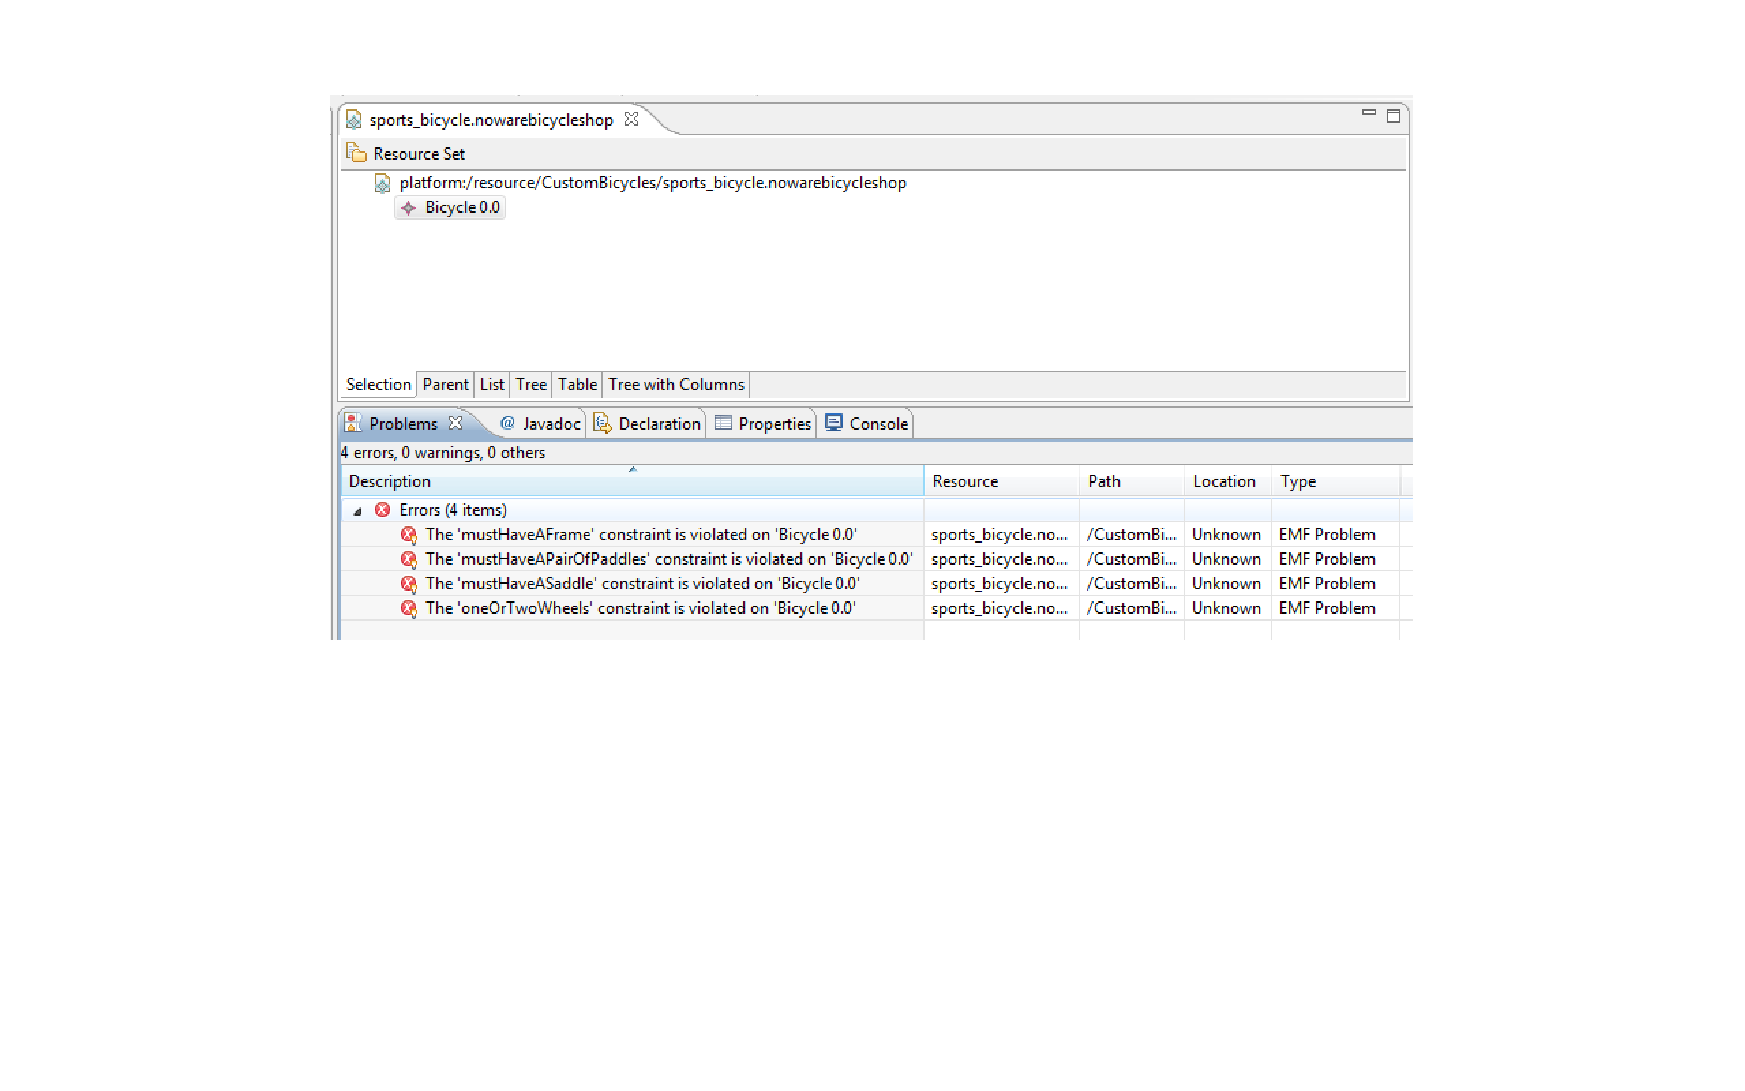
\includegraphics[width=\textwidth]{fig/ocl_examples/ocl_bicycle_model_errors.pdf}
        \caption{OCL constraints violated in a bicycle: no frame, no padles, no
        saddle, no wheel}
        \label{fig.ocl_bike_errors}
    \end{center}
\end{figure}

\begin{figure}[H]
    \begin{center}
        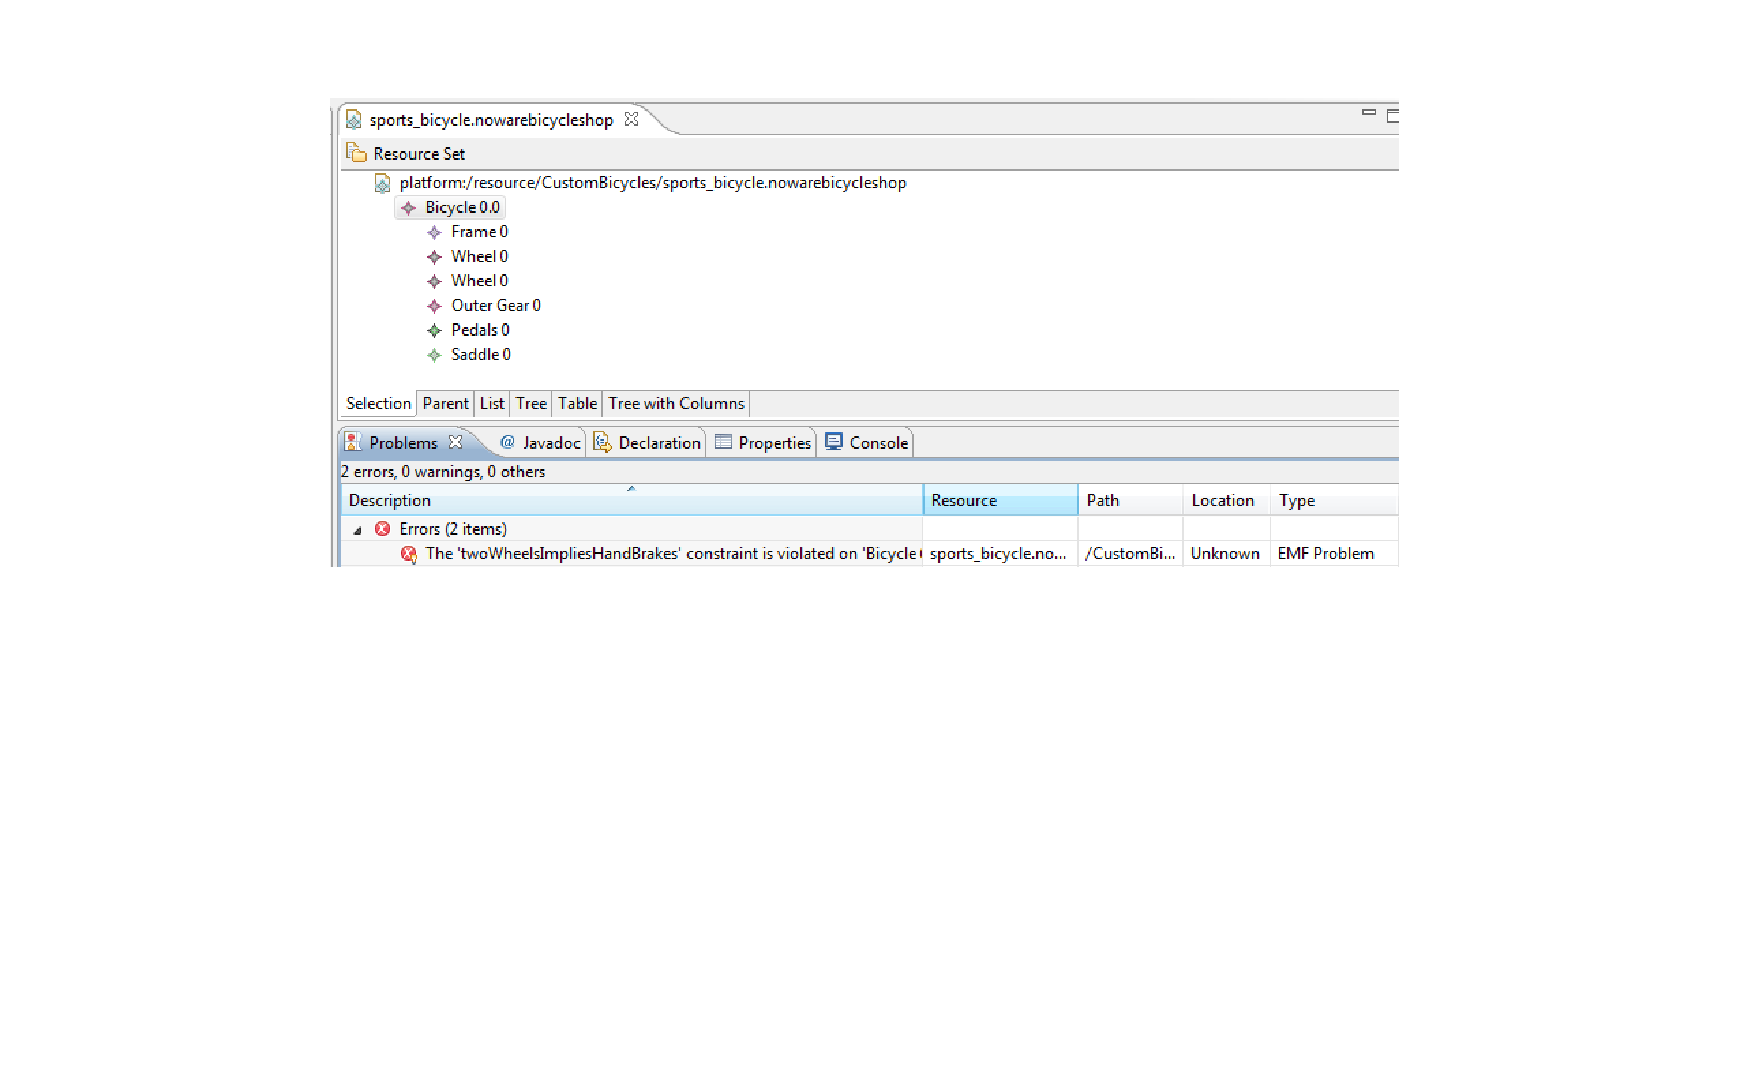
\includegraphics[width=\textwidth]{fig/ocl_examples/ocl_sports_bicycle_wheel_constraint_errors.pdf}
        \caption{OCL constraint violated in sports bicycle: two wheel imply
        hand brakes}
        \label{fig.ocl_ecore_handbreaks}
    \end{center}
\end{figure}

\subsection{Examples of errors in GMF}

\begin{figure}[H]
    \begin{center}
        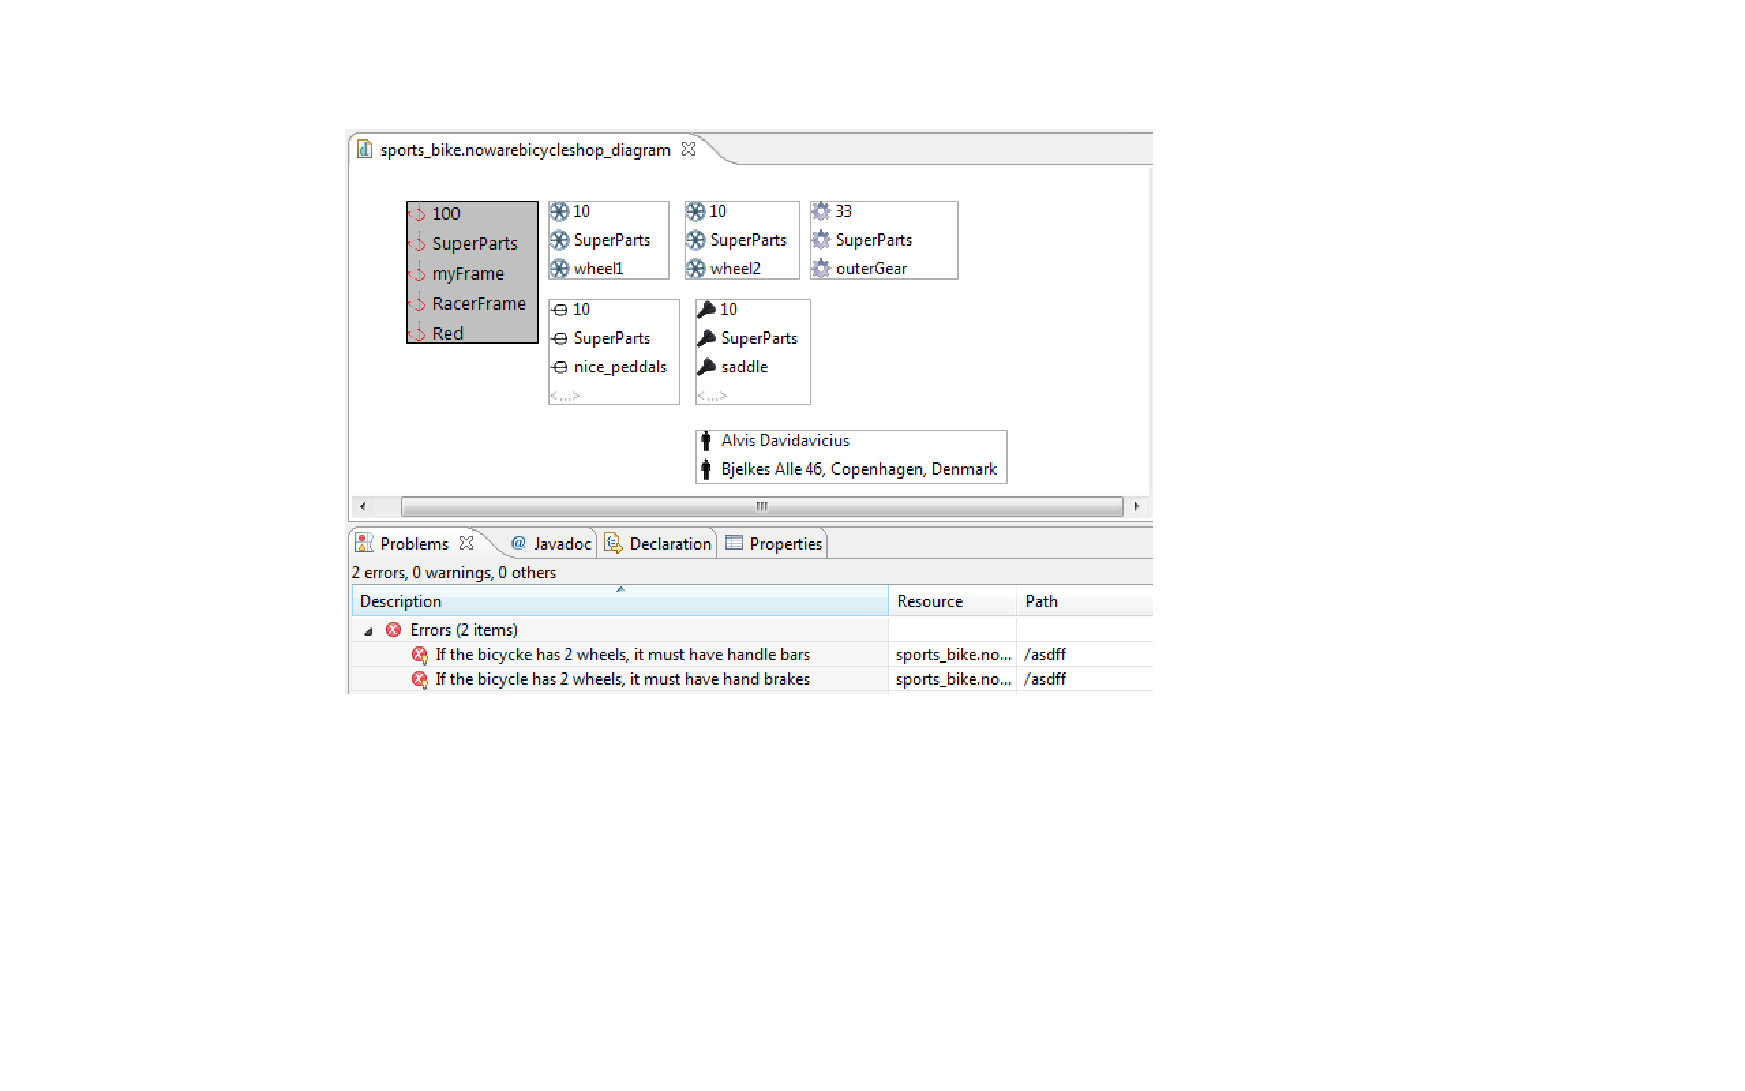
\includegraphics[width=\textwidth]{fig/gmf/validation/validation_example.pdf}
        \caption{Example of validation in GMF: pretty-printed messages}
        \label{fig.gmf_validation}
    \end{center}
\end{figure}
